\chapter{Risk factors: fruits}
\label{applications-log_normal}

Within the GBD 2010 Study, the meta-regression framework constructs an age-sex pattern for risk factor exposures.  Risk factors affect disease outcomes.

Fruit consumption is a risk factor that has a significant protective effect against morbidity and mortality from several diseases.  Fruit consumption is measured as the total intake of fruit per day.  Fruit includes all fresh, frozen, cooked, canned or dried fruits, excluding fruit juices and salted or pickled fruits. \cite{he_increased_2007, boeing_intake_2006}

National and subnational surveys and dietary studies provided measurement of total fruit intake via diet recalls, diet records, food frequency questionnaires and household availability or budget surveys.  After rejecting data without measures of uncertainty, a total of 1502 rows of data representing 104 countries were included for analysis.

Often it is useful to design statistical models based on real world processes, using count models for discrete data and rate models for continuous data as discussed in Chapter \ref{theory-rate_model}.  Since fruit consumption is a continuous variable, one may choose the log normal or normal rate model over the negative binomial model to maintain a mechanistic understanding of the statistical model.  The models differ in their treatment of numbers that are very close to zero, but choice of rate model does not impact the estimate, especially with well behaved data, as seen in Figure \ref{fig:app-fruit rate type}.

    \begin{figure}[h]
        \begin{center}
            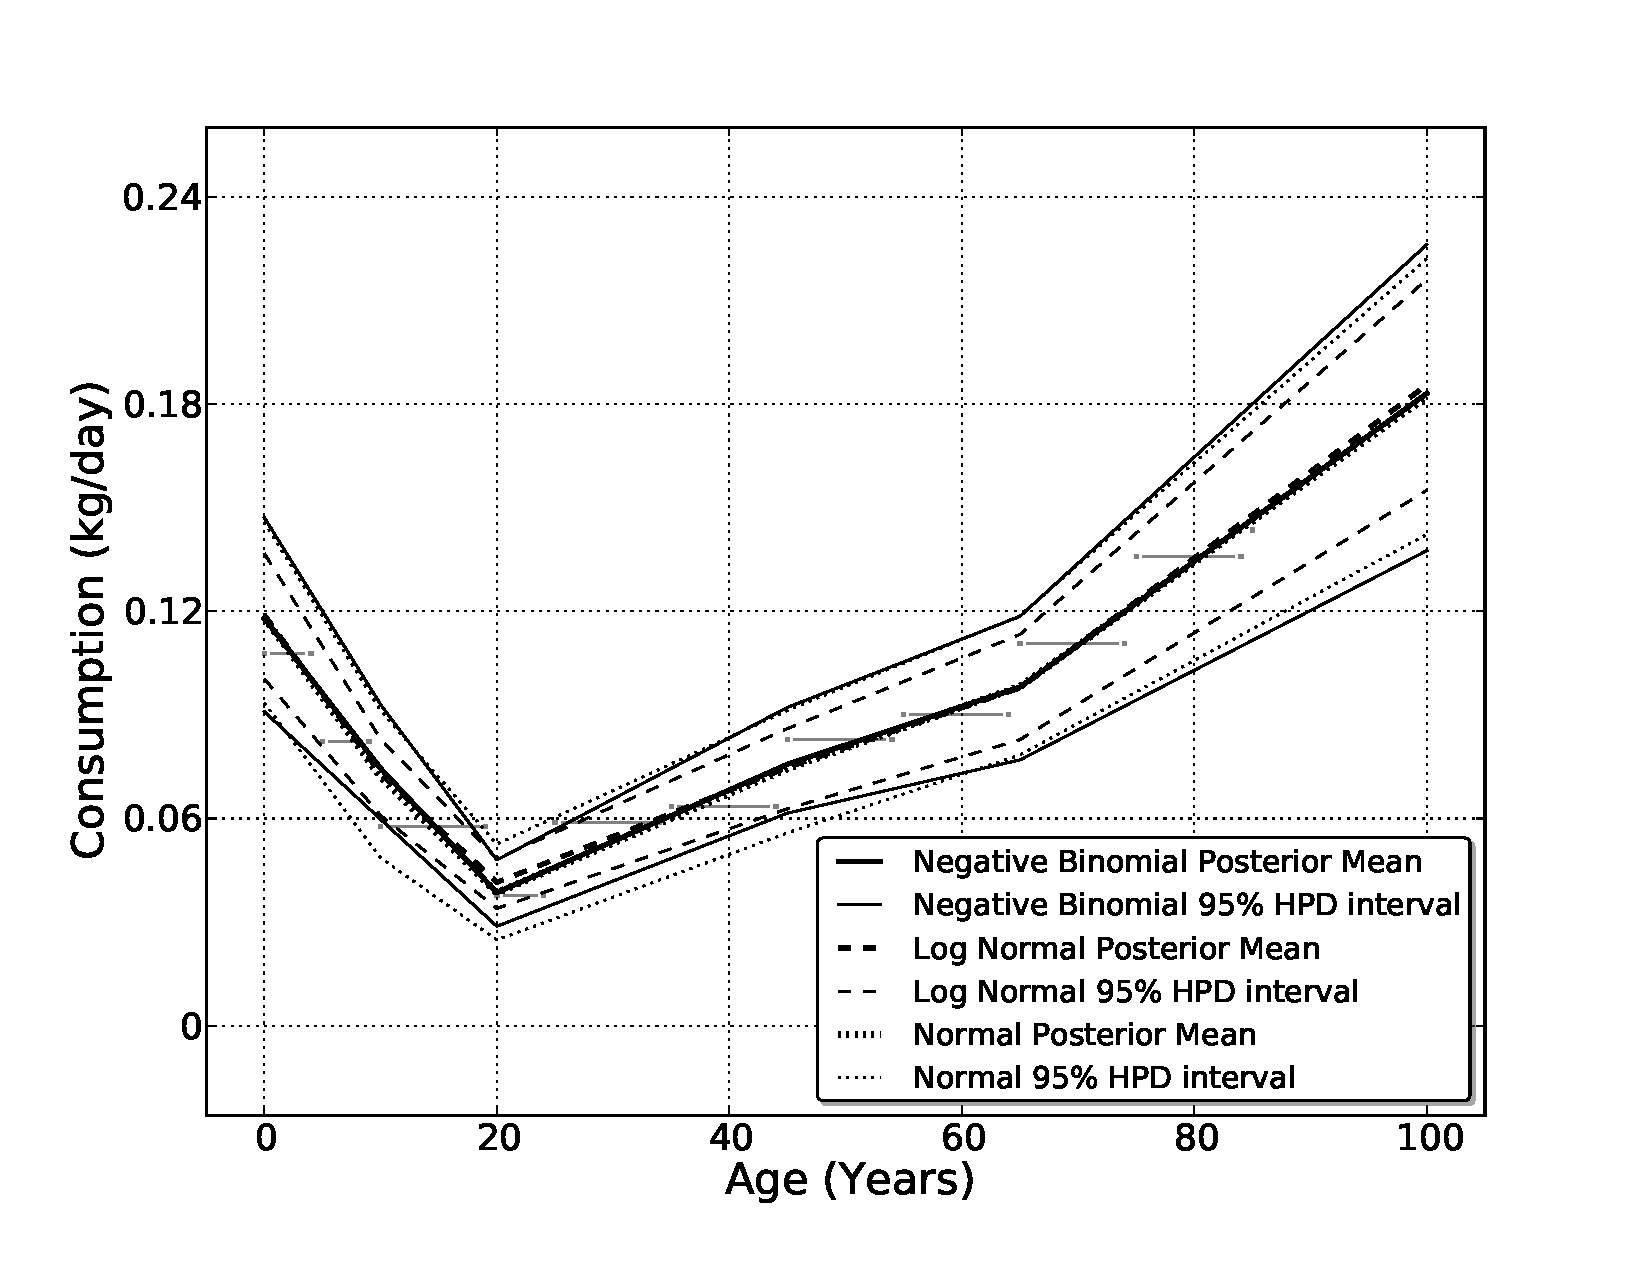
\includegraphics[width=\textwidth]{fruit-rate_type.pdf}
            \caption{Comparison of fruit consumption estimates in males in the United States of America in 2005 using the negative binomial, log normal and normal rate models.}
            \label{fig:app-fruit rate type}
        \end{center}
    \end{figure} 